\documentclass[10pt]{article}

% Preamble

\usepackage{amsmath,amsfonts,amssymb}
\usepackage[mathscr]{euscript}
%\usepackage[mathcal]{euscript}
\usepackage{mathrsfs}
\usepackage{graphicx}
\usepackage{float}
\usepackage{bbm}
\usepackage{braket}
\usepackage{tikz-feynman}
\usepackage{simpler-wick}
\usepackage{cancel}
\usepackage{stackengine}
\usepackage{slashed}

\newcommand{\bigzero}{\mbox{\normalfont\Large\bfseries 0}}

\title{Notes On Relativistic Quantum Field Theory: \\ A Course Given By Dr. Tobias Osborne \\ Part II: The Dirac Field}
\author{Transcribed by Dr. Alexander V. St. John}

% The Document

\begin{document}

\maketitle

\clearpage

\section*{Lecture 14: The Dirac Field}
\label{sec:lec14}


\noindent We've built a relativistic quantum field theory for the (complex) scalar field, or spinless particles, around the Klein-Gordon equation and its Lorentz group invariant, conserved quantities, or the generators of Lorentz transformations (e.g., boosts and rotations), which obey the Lie algebra bracket

\begin{equation}
[J^{\rho \sigma}, J^{\tau \nu}] = \eta^{\sigma \tau} J^{\rho\nu} - \eta^{\rho \tau} J^{\sigma \nu} + \eta^{\rho\nu} J^{\sigma \tau} - \eta^{\sigma \nu} J^{\rho \tau} .
\end{equation} 

\noindent We now build a relativistic quantum field theory for fermions, particles of spin-$\frac{1}{2}$, which requires a (complex) vector, or spinor, field to describe the dynamics of the fermionic field. Our strategy is similar to the scalar field case:

\begin{itemize}
\item Build a relativistic classical field theory.
\item Quantize the field (by guess).
\item Check for the (projective) representation of the Lorentz group.
\end{itemize}

\noindent To begin with building the relativistic classical field theory, given a set of objects obeying the Lie bracket above, we construct a Lagrangian by first constructing the representation of the Lorentz group via $g=e^{-\frac{i}{2} \omega_{\mu\nu}J^{\mu\nu}}$, where $\omega_{\mu\nu}$ are the Lorentz boost parameters, and then calculating Lagrangian densities invariant under the representation $g$.

\subsection*{Dirac's Motivation}

\noindent Dirac desired to factorize the Klein-Gordon equation, and craft an equation of motion linear in spacetime derivatives $\partial_\mu \equiv \partial / \partial x^\mu$, the square root of the Klein-Gordon equation, such that any solution to the Dirac equation is also a solution to the Klein-Gordon equation, but not necessarily vice versa. Linearity in the spacetime derivatives ensures that the associated probability current is positive definite, and the positive energy solutions may be separated from the negative energy solutions inherent to solutions of the Klein-Gordon equation. \\

\noindent The Dirac equation, which we will motivate and derive, reads

\begin{equation}
(i \gamma^\mu \partial_\mu - m) \psi = 0 .
\end{equation}

\noindent Where the coefficients of the spacetime derivatives $i\gamma^\mu$ can not be just four scalar quantities, as the vector of coefficients would then define a direction, and the Dirac equation would not be Lorentz invariant. The $\gamma^\mu$ must actually be $4\times 4$ matrices, and the field $\psi$ must be a four-vector. \\

\noindent To recover the Klein-Gordon equation from the Dirac equation, multiply the Dirac equation by $(i \gamma^\nu \partial_\nu + m)$, and compare to the Klein-Gordon equation $(\partial^2 + m^2)\psi=0$ to see that the "squared" Dirac equation becomes the Klein-Gordon equation if the \textit{gamma matrices} obey the following anticommutation relation

\begin{equation}
\{ \gamma^\mu, \gamma^\nu \} = 2 \eta^{\mu\nu} \cdot \mathbb{I}_{n \times n}.
\end{equation}

\noindent Where $\eta^{\mu\nu}$ is the Minkowski metric tensor.

\subsection*{Generators of Fermionic Field (Lorentz) Transformations}

\noindent To calculate the generators of the Lorentz transformations of the fermionic field (spin-$\frac{1}{2}$ particles), suppose that we have that set of 4 $n \times n$ matrices $\gamma^\mu$ that satisfy the anticommutation relation $\{ \gamma^\mu, \gamma^\nu \} = 2 \eta^{\mu\nu} \cdot \mathbb{I}_{n \times n}$. Obtain a solution in terms of the gamma matrices that obeys the Lie algebra bracket above

\begin{equation}
J^{\mu\nu} \to S^{\mu\nu} \equiv \frac{i}{4} [\gamma^\mu, \gamma^\nu].
\end{equation}

\noindent It is an \textbf{(exercise)} to check that these generators obey Lie algebra bracket above for the Lorentz transformation, and that four dimensions is the minimum of the gamma matrices dimensionality for nontrivial solutions. \\

\noindent The gamma matrices that correctly form the Lorentz group in $(3+1)$d spacetime were crafted by Dirac via the Pauli spin (sigma) matrices

\begin{equation}
\gamma^0 = \left( \begin{array}{c|c} 0 & \mathbb{I} \\ \hline \mathbb{I} & 0 \end{array} \right) \,\,\,\,\,\,\,\, \gamma^j = \left( \begin{array}{c|c} 0 & \sigma^j \\ \hline -\sigma^j & 0 \end{array} \right) .
\end{equation}

\noindent Where the Pauli sigma matrices read
\begin{equation}
\sigma^1 = \left( \begin{array}{cc} 0 & 1 \\ 1 & 0 \end{array} \right) \,\,\,\, \sigma^2 = \left( \begin{array}{cc} 0 & -i \\ i & 0 \end{array} \right) \,\,\,\, \sigma^3 = \left( \begin{array}{cc} 1 & 0 \\ 0 & -1 \end{array} \right) .
\end{equation}

\noindent The timelike components $S^{0j}$ yield three ($j=1,2,3$) boost generators of the Lorentz group (of the Lie algebra above)
\begin{equation}
S^{0j} = \frac{i}{4} \left[ \gamma^0, \gamma^j \right] = -\frac{i}{2} \left(\begin{array}{cc} \sigma^j & 0 \\ 0 & -\sigma^j \end{array} \right) .
\end{equation}

\noindent The other six generators from the spacelike components have the form
\begin{equation}
S^{jk} = \frac{i}{4} \left[ \gamma^j, \gamma^k \right] = \frac{1}{2} \epsilon^{jkl} \left(\begin{array}{cc} \sigma^l & 0 \\ 0 & -\sigma^l \end{array} \right)
\end{equation}

\noindent Where the sigma matrices obey the commutation relation: $[\sigma^j,\sigma^k] = 2i\epsilon^{jkl} \sigma^l$. \\

\subsection*{Construction of Gamma Matrices}

\noindent To build the operators that obey the desired anticommutation relation, and also form a \textit{Clifford algebra}, implement the \textbf{Jordan-Wigner transformation}, which maps the Pauli sigma matrices to fermionic creation and annihilation operators.

\subsubsection*{Jordan-Wigner Transformation}

\noindent Suppose that you want to represent operators that obey the (fermionic) anticommutation relation
\begin{equation}
\{\mu^a, (\mu^b)^\dagger\} = \delta^{ab}, \,\,\,\, a,b \, = \, 1,2,\dots,n.
\end{equation}

\noindent Consider the operator $\sigma^+ = \left(\begin{array}{cc} 0 & 0 \\ 1 & 0 \end{array} \right)$, and the construction of successive operators which all operate on the same $n$-dimensional space, permissing the expanse of $n$ direct products with the unit operator
\begin{align*}
\mu^1 &= \sigma^+ \otimes \mathbb{I} \otimes \mathbb{I} \otimes \mathbb{I} \otimes \mathbb{I} \otimes \dots \otimes \mathbb{I} \\
\mu^2 &= \sigma^3 \otimes \sigma^+ \otimes \mathbb{I} \otimes \mathbb{I} \otimes \mathbb{I} \otimes \dots \otimes \mathbb{I} \\
\mu^3 &= \sigma^3 \otimes \sigma^3 \otimes \sigma^+ \otimes \mathbb{I} \otimes \mathbb{I} \otimes \dots \otimes \mathbb{I} \\
\mu^4 &= etc. \, \dots
\end{align*}

\noindent These $\mu^j$ operators obey the fermioic anticommutation relations, since $\{\sigma^j, \sigma^k \} = 2 \delta^{jk}$, and form a matrix representation of the anticommutation relation given in the Jordan-Wigner transformation.

\noindent An inefficient method to construct a representation of the gamma matrices, though reducible to the above $\mu^j$ matrices, which honors the anticommutation relation, starts with the composition of the timelike gamma matrix
\begin{equation}
\gamma^0 = \sigma^1 \otimes \mathbb{I} .
\end{equation}

\noindent Next, we know that $\sigma^2$ anticommutes with $\sigma^1$ via $\{\sigma^j, \sigma^k \} = 2 \delta^{jk}$, and thus we construct the following, noting that to satisfy $(\gamma^j)^2 <0$, scalar multiplication by the imaginary unit $i$ is required
\begin{equation}
\gamma^j \equiv i \sigma^2 \otimes \sigma^j .
\end{equation}

\subsection*{The Dirac Spinor}

\noindent The set of matrices $\gamma^\mu$ satisfying the anticommutation relation $\{ \gamma^\mu, \gamma^\nu \} = 2 \eta^{\mu\nu} \cdot \mathbb{I}_{n \times n}$ are called the \textbf{Dirac matrices}, and the four-component object that transforms correctly under the Lorentz group is called the \textbf{Dirac spinor}
\begin{equation}
\psi \to e^{-\frac{i}{2} \omega_{\mu\nu} S^{\mu\nu}} \psi
\end{equation}
This is the definition of the spinor in different reference frames, and defines the \textbf{spinor field} as a mapping
\begin{equation}
\psi: \mathbb{R}^{1,3} \to \mathbb{C}^4.
\end{equation}

\noindent Transforming as
\begin{equation}
\psi_a(x) = \sum_{b=0}^3 [ \Lambda_{1/2} ]_{ab} \,\, \psi_b(\Lambda^{-1}x), \,\, \Lambda \in SO(3)
\end{equation}

\noindent Where $\Lambda$ is the usual representation for the Lorentz transformation, and $\Lambda_{1/2}$ has the same representation structure and obeys the same Lie algebra of the Lorentz transformation, but different elements: the $4\times4$ matrix Lie algebra bracket $S^{\mu\nu}$ built out of the gamma matrices
\begin{align}
\Lambda &= e^{-\frac{i}{2} \omega_{\mu\nu} J^{\mu\nu}} \\
\Lambda_{1/2} &= e^{-\frac{i}{2} \omega_{\mu\nu} S^{\mu\nu}}
\end{align}

\noindent Every representation of the Lorentz group can be used to build Lorentz invariant field equations, such that $\mathcal{D}\psi=0$. To build the field equations for $\psi_a(x)$, first guess and check (\textbf{Exercise}) that the Klein-Gordon equation is satisfied
\begin{equation}
(\partial^2 + m^2) \psi_a(x) = 0, \, \forall \, a
\end{equation}

\noindent The next guess, by Dirac, is to find a satisfactory field equation that is linear in spacetime derivatives. This requires the following identity as an auxiliary computation between the gamma matrices and the two generators, first confirmed by Dirac (\textbf{Exercise})
\begin{equation}
[\gamma^\mu, S^{\rho\sigma}] = (J^{\rho\sigma})^\mu_{\,\,\,\nu} \, \gamma^\nu
\end{equation}

\noindent This is reminiscient of how the four-vector transforms under the Lorentz transformation, and we motivatedly write, to first order in $\omega$
\begin{align}
(1+\frac{i}{2}  \omega_{\rho\sigma} S^{\rho\sigma}) \gamma^\mu (1-\frac{i}{2}  \omega_{\rho\sigma} S^{\rho\sigma}) &= (1-\frac{i}{2}  \omega_{\rho\sigma} J^{\rho\sigma})^\mu_{\,\,\,\nu} \gamma^\nu \\
e^{\frac{i}{2} \omega_{\rho\sigma} S^{\rho\sigma}} \gamma^\mu e^{-\frac{i}{2} \omega_{\rho\sigma} S^{\rho\sigma}} &\approx (e^{-\frac{i}{2} \omega_{\rho\sigma} J^{\rho\sigma}})^\mu_{\,\,\,\nu} \gamma^\nu  \\
\Lambda_{1/2}^{-1} \gamma^\mu \Lambda_{1/2} &= \Lambda^\mu_{\,\,\,\nu} \gamma^\nu
\end{align}

\noindent This shows that the gamma matrices transform exactly like a four-vector under the Lorentz transformation. Contracted against another vector, that transforms accordinngly, will produce another Lorentz invariant object. The differential operator $\partial_\mu$ transforms as such, making $\gamma^\mu \partial_\mu$ Lorentz invariant. \\

\noindent Thus, the Lorentz invariant field equation, the Dirac equation, reads
\begin{equation}
(i\gamma^\mu \partial_\mu - m) \psi = 0
\end{equation}

\noindent Check the invariance of the Dirac equation by substituting the following quantities for the spinor and spacetime derivative into the Dirac equation (\textbf{Exercise})
\begin{align}
\psi(x) &\to \Lambda_{1/2} \psi \, (\Lambda^{-1}x) \\
\partial_\mu &\to (\Lambda^{-1})^\nu_{\,\,\,\mu} \partial_\nu .
\end{align}

\noindent Making these subsitutions, the Dirac equation becomes
\begin{align}
\left( i\gamma^\mu (\Lambda^{-1})^\nu_{\,\,\,\mu}\partial_\nu - m \right) \Lambda_{1/2}\, \psi(\Lambda^{-1}x) &= 0 \\
\Lambda_{1/2} \Lambda^{-1}_{1/2}\cdot \left( i\gamma^\mu (\Lambda^{-1})^\nu_{\,\,\,\mu}\partial_\nu - m \right) \Lambda_{1/2}\, \psi(\Lambda^{-1}x) &= 0 \\
\Lambda_{1/2}\, \left( i\Lambda^{-1}_{1/2}\,\gamma^\mu \Lambda_{1/2} \,(\Lambda^{-1})^\nu_{\,\,\,\mu}\partial_\nu - m \right) \psi(\Lambda^{-1}x) &= 0 \\
\Lambda_{1/2}\, \left( i\Lambda^\mu_{\,\,\,\sigma} \gamma^\sigma (\Lambda^{-1})^\nu_{\,\,\,\mu}\partial_\nu - m \right) \psi(\Lambda^{-1}x) &= 0 \\
\Lambda_{1/2}\, \left( i\gamma^\nu \partial_\nu - m \right) \psi(\Lambda^{-1}x) &= 0 
\end{align}

\noindent Going from line 2 to 3 utilizes the fact that $(\Lambda^{-1})^\nu_{\,\,\,\mu}\partial_\nu$ is a linear operator, meaning the quantity $\Lambda^{-1}_{1/2}\,\gamma^\mu \Lambda_{1/2}$ also transforms like a four-vector and is Lorentz invariant. Going from line 4 to 5 uses the fact that $(\Lambda^{-1})^\nu_{\,\,\,\mu}\partial_\nu \, \psi(\Lambda^{-1} x)$ is a delta function. The left hand side becomes zero, and the Dirac equation is Lorentz invariant. \\

\noindent The Dirac equation contains the Klein-Gordon equation
\begin{align*}
(i\gamma^\mu \partial_\mu - m) \psi &= 0 \\
(-i\gamma^\nu \partial_\nu - m) \cdot (i\gamma^\mu \partial_\mu - m) \psi &= 0 \\
(\frac{1}{2} \{ \gamma^\mu, \gamma^\nu \} \partial_\mu \partial_\nu + m^2)\psi &= 0 \\
(\partial^\mu \partial^\nu + m^2) \psi &= 0 \\
(\Box^2 + m^2) \psi &= 0
\end{align*}

\noindent The Dirac equation is first order in all four spacetime coordinates, and is thus a stronger condition imposed on the components of the field $\psi$. 

\clearpage

\section*{Lecture 15: The Dirac Equation and its Solutions}
\label{sec:lec15}

\noindent The Dirac equation $\left( i \gamma^{\mu} \partial_{\mu} - m \right) \psi = 0$ is motivated for us by the question of the dynamics of fermionic fields, espeically electrons. We introduce a new representation of the Lorentz group with intrinsic angular momentum by producing the gamma matrices $\gamma^{\mu}$, such that the anticommutation relation is satisfied. 

\begin{equation}
\{ \gamma^{\mu}, \, \gamma^{\nu} \} = \eta^{\mu\nu} \cdot \mathbb{I}
\end{equation}

\noindent And recall that the gamma matrices contain the Pauli spin matrices and have the form

\begin{equation}
\gamma^0 = \left( \begin{array}{c|c} 0 & \mathbb{I} \\ \hline \mathbb{I} & 0 \end{array} \right) \,\,\,\,\,\,\,\, \gamma^j = \left( \begin{array}{c|c} 0 & \sigma^j \\ \hline -\sigma^j & 0 \end{array} \right) .
\end{equation}

\noindent This will yield a new Lorentz-invariant equation of motion, and the steps to get there include

\begin{enumerate}
\item Calculating the Hamiltonian denisty from the Lagrangian density and guessing a quantization.
\item Entering the zero-mass limit, where the equation of motion decouples.
\item Solve the wave equation in the free particle basis.
\end{enumerate}

\noindent Recall that the Dirac spinor Lorentz-transforms according to 

\begin{equation}
\psi(x) \rightarrow \Lambda_{1/2} \psi (\Lambda^{-1} x)
\end{equation}

\noindent To build the Lagrangian density, we need to define some Lorentz scalars. A first guess may be to (incorrectly) define the Lorentz scalar as the quantity $\psi^\dagger (x) \psi (x)$, which Lorentz transforms as

\begin{equation}
\psi^\dagger (x) \psi (x) \rightarrow \psi^\dagger \Lambda_{1/2} ^\dagger \Lambda_{1/2} \psi
\end{equation}

\noindent The issue with this definition is that the representation of the Lorentz group can be unitary if it is finite dimensional, and, in general, $\Lambda_{1/2} ^\dagger \Lambda_{1/2}  \ne \mathbb{I}$, and $\Lambda_{1/2}$ is not unitary. The proper definition of the Lorentz scalar includes a gamma matrix factor to ensure unitarity. \\

\noindent  Define the Lorentz scalar as $\psi^\dagger (x) \gamma ^0 \psi (x)$, and define the quantity $\bar{\psi}(x) = \psi^\dagger (x) \gamma ^0$ to assist in proving that $\bar{\psi}\psi$ is indeed a Lorentz scalar.  \\

\noindent \textbf{Exercise}: Prove this using the \\

\textbf{Lemma}: $\Lambda_{1/2} ^\dagger \gamma^0 = \gamma^0 \Lambda_{1/2} ^{-1}$. \\

\noindent Similarly, define the Lorentz vector $v^\mu = \bar{\psi} \gamma^\mu \psi$. \\

\noindent Therefore, the Lagrangian density for the Dirac field is

\begin{equation}
\mathcal{L}_{Dirac} = \bar{\psi} \left( i \gamma^\mu \partial_\mu - m \right) \psi
\end{equation}

\noindent \textbf{Exercise}: Prove that $\mathcal{L}_{Dirac}$ is Lorentz scalar. \\
\noindent \textbf{Exercise}: Apply the Euler-Lagrange equation to obtain the Dirac equation. \\

\subsection*{Dirac Field Hamiltonian}

\noindent The conjugate momentum to the Dirac spinor $\psi$ is the quantity $i \psi^\dagger$, yielding the Hamiltonian

\begin{align}
H &= \int d^3 x \,\, \bar{\psi} \left( -i \underline{\gamma} \cdot \underline{\nabla} + m \right) \psi \\
H &= \int d^3 x \,\, \psi^\dagger \left( -i \gamma^0 \underline{\gamma} \cdot \underline{\nabla} + m \gamma^0 \right) \psi
\end{align}

\noindent Where the underlined vectors are only the spatial components, such that 
$$\underline{\gamma} \cdot \underline{\nabla}  = \sum_{j=1}^3 \gamma^j \partial_j.$$

\noindent And we have the dynamics of a classical Dirac field.

\subsection*{Zero-mass Limit}

\noindent Let's see how the Dirac equation and the four-component Dirac spinor decouples in the zero-mass limit to the two-component \textit{Weyl spinors} $\psi_{L/R}(x) \in \mathbb{C}^2$.

\begin{equation}
\psi(x) = \left( \begin{array}{c} \psi_1(x) \\ \psi_2(x) \\ \psi_3(x) \\ \psi_4(x) \end{array} \right) \rightarrow \left( \begin{array}{c}\psi_L(x) \\ \psi_R(x) \end{array} \right)
\end{equation}

\noindent Under the Lorentz transformation, Weyl spinors transform to themselves

\begin{align}
\psi_L &\rightarrow (\mathbb{I} - i \underline{\theta} \cdot \frac{1}{2} \underline{\sigma} - \underline{\beta} \cdot \frac{1}{2} \underline{\sigma} ) \psi_L \\
\psi_R &\rightarrow(\mathbb{I} - i \underline{\theta} \cdot \frac{1}{2} \underline{\sigma} + \underline{\beta} \cdot \frac{1}{2} \underline{\sigma} ) \psi_R
\end{align}

\noindent Where the rotation and boost three-vectors are, respectively, $\underline{\theta} = (\theta_1,\theta_2,\theta_3)$ and $\underline{\beta} = (\beta_1,\beta_2,\beta_3)$. \\

\noindent The left-handed spinor $\psi_L$ contains the right-handed spinor $\psi_R$, seen by taking the complex conjugate and multiplying by $\sigma^2$, since this causes a \textit{spin flip}, such that multiplication by $\sigma^2$ give the antipode on the Bloch sphere.

\begin{equation}
\sigma^2 \underline{\sigma}^* = - \underline{\sigma} \sigma^2
\end{equation}

\noindent Therefore, the quantity $\sigma^2 \psi_L^*$ transforms like $\psi_R$. \\

\noindent The coupling of the Weyl spinors is represented by the matrix equation (\textbf{Exercise})

\begin{equation}
\left( i \gamma^\mu \partial_\mu - m \right) \psi = \left( \begin{array}{cc} -m & i(\partial_0 + \underline{\sigma} \cdot \underline{\nabla}) \\ i(\partial_0 - \underline{\sigma} \cdot \underline{\nabla}) & m \end{array} \right) \left( \begin{array}{c} \psi_L \\ \psi_R \end{array} \right) = 0
\end{equation}

\noindent Now, suppose that $m=0$, such that $\psi_L$ and $\psi_R$ become two independent solutions to the Dirac equation, and we obtain a represntation of the Poincar\'e group. The equations of motion in the zero-mass limit are then

\begin{align}
i (\partial_0 - \underline{\sigma} \cdot \underline{\nabla} ) \psi_L &= 0 \\
i (\partial_0 + \underline{\sigma} \cdot \underline{\nabla} ) \psi_R &= 0 
\end{align}

\noindent Define the notation

\begin{align}
\sigma^\mu &= (1, \underline{\sigma}) \\
\bar{\sigma}^\mu &= (1, -\underline{\sigma})
\end{align}

\noindent Then the gamma matrices become

\begin{equation}
\gamma^\mu = \left( \begin{array}{cc} 0 & \sigma^\mu \\ \bar{\sigma}^\mu & 0 \end{array} \right)
\end{equation}

\noindent And we rewrite the Dirac equations of motion as

\begin{align}
i (\bar{\sigma} \cdot \partial) \psi_L &= 0 \\
i (\sigma \cdot \partial) \psi_R &= 0 
\end{align}

\subsection*{Free Particle Solutions to the Dirac Equation}

\noindent The Dirac equation is a linear system of partial differental equations (PDEs), and the solutions may be expressed in terms of plane waves

\begin{equation}
\psi(x) = e^{-i p \cdot x} u(p)
\end{equation}

\noindent Where $u(p) \in \mathbb{C}^4$ and are the zero eigenvectors of the Dirac matrix. Linear combinations of $\psi(x)$ yield a general solution, with the constraint of \textit{on-shell momentum}, such that $p^2 = m^2, \, p^0 > 0$. \\

\noindent Substitute the plane wave solution in to Dirac equation to obtain the matrix equation

\begin{equation}
(p_\mu \gamma^\mu - m \cdot \mathbb{I}) \, u(p) = 0
\end{equation}

\noindent Now, solving for $u(p)$, enter the rest frame, where $p_0 = (m,0)$, and the matrix equation becomes

\begin{equation}
\left( m \left( \begin{array}{cc} 0 & \mathbb{I} \\ \mathbb{I} & 0 \end{array} \right) - m \left( \begin{array}{cc} \mathbb{I} & 0 \\ 0 & \mathbb{I} \end{array} \right)  \right) \left( \begin{array}{c} u_L(p_0) \\ u_R(p_0) \end{array} \right) = 0
\end{equation}

\noindent And solutions are of the form

\begin{equation}
u_L(p_0) = u_R(p_0) = \sqrt{m} \, \xi
\end{equation}

\noindent Where $\xi$ fixed, with normalization $\xi^\dagger \xi = 1$. Then the solution in the rest frame is 

\begin{equation}
\psi^s(x) = e^{-i p \cdot x} u^s(p_0) = \sqrt{m} \left(\begin{array}{c} \xi^s \\ \xi^s \end{array} \right) e^{-i p \cdot x}
\end{equation}

\noindent Where $s=1,2$, and we may write $\xi^1 = \left( \begin{array}{c} 1 \\ 0 \end{array} \right)$ and $\xi^2 = \left( \begin{array}{c} 0 \\ 1 \end{array} \right)$.

\noindent The solution in a general reference frame is obtained via the spinor representation of the Lorentz boost $\Lambda$. To calculate the spinor representation of the Lorentz boost along any three-direction, recall that, for rapidity $\eta$

\begin{align}
\Lambda &= \cosh (\eta) \cdot \mathbb{I} + \sinh(\eta) \cdot \left( \begin{array}{cccc} 0&0&0&1\\0&0&0&0\\0&0&0&0\\1&0&0&0 \end{array} \right) \\
&= e^{-i \frac{1}{2} \omega_{\mu\nu} J^{\mu\nu}} \\
\Lambda &= e^{-i \frac{1}{2} \omega_{0 3} J^{0 3} }
\end{align}

\noindent Where $J^{\mu\nu}$ obey the Lie algebra of the Lorentz group, $\omega_{\mu\nu}$ are the 6 boost parameters, and $\omega_{0 3}=2\eta$ is the only nonzero term (\textbf{Exercise}).

\noindent To apply this transformation on the spinor, apply the matrix

\begin{align}
\Lambda_{1/2} &= e^{-\frac{i}{2} \omega_{03} S^{03} }\\
&= e^{-\frac{i}{2} \cdot 2 \eta \cdot \frac{i}{4} [ \gamma^0, \, \gamma^3 ]} \\
&= \left( \begin{array}{cc} e^{-\frac{1}{2} \eta \sigma^3} & 0 \\ 0 & e^{\frac{1}{2} \eta \sigma^3} \end{array} \right) 
\end{align}

\noindent So, in the general reference frame, $p=\Lambda p_0$, the solutions have the form (\textbf{Exercise})

\begin{align}
\psi(x) &= e^{-i p \cdot x} u^s(p=\Lambda p_0) \\
&= \sqrt{m} \left( \begin{array}{c} e^{-\frac{1}{2} \eta \sigma^3} \xi^s \\ e^{\frac{1}{2} \eta \sigma^3} \xi^s \end{array} \right) e^{-i p \cdot x} \\
&= \left( \begin{array}{c} \sqrt{p\cdot \sigma} \xi^s \\ \sqrt{p \cdot \bar{\sigma}} \xi^s \end{array} \right) e^{-i p \cdot x}
\end{align}

\noindent Where we used $(p \cdot \sigma)(p \cdot \bar{\sigma}) = m^2 = p^2$, and we have two linearly independent solutions to the Dirac equation, but we need four solutions per given momentum. 

\noindent The other two solutions come from the \textit{plane wave ansatz} for the negative frequency solutions.

\begin{equation}
\psi_{negative}(x) = v(p) e^{i p \cdot x}
\end{equation}

\noindent Similar to the positive frequency case, there are two linearly independent solutions

\begin{align}
\psi_{negative} (x) &= e^{i p \cdot x} v^s (p) \\
&= \left( \begin{array}{c} \sqrt{p\cdot \sigma} \xi^s \\ -\sqrt{p \cdot \bar{\sigma}} \xi^s \end{array} \right) e^{i p \cdot x}
\end{align}

\noindent To normalize these states, recall that $\bar{\psi}\psi$ is Lorentz invariant, with $\psi(x) = u^s(p) e^{-ip \cdot x}$, such that 

\begin{equation}
\bar{\psi} \psi = \bar{u}^s (p) u^s (p) = 2 m (\xi^s)^\dagger \xi^s
\end{equation}

\noindent And more generally, for both positive and negative frequency solutions

\begin{align}
\bar{\psi} \psi &= \bar{u}^r (p) u^s (p) = 2 m \delta^{rs} \\
\bar{\psi}_{negative} \psi_{negative} &= \bar{v}^r (p) v^s (p) = -2 m \delta^{rs}
\end{align}

\noindent And for mixed positive-negative frequency solutions, the normalization is zero

\begin{equation}
\bar{u}^r(p) v^s (p) = \bar{v}^r (p) u^s (p) = 0
\end{equation}

\noindent There we have four linearly independent solutions to the (classical) Dirac equation in a general reference frame. 

\clearpage

\section*{Lecture 16: The Quantum Dirac Field}
\label{sec:lec16}


\noindent In the last lecture we found plane wave solutions to the classical Dirac equation. Now, we will guess a (quadractic) quantum theory that begins with the plane wave solutions of an effective classical theory in its large scale, low energy, high decoherence limit. The classical theory we make our guess has the Lagrangian density 

\begin{equation}
\mathcal{L} = \bar{\psi} (i \slashed{\partial} - m \cdot \mathbb{I} ) \psi = \bar{\psi} (i \gamma^\mu \partial_\mu - m \cdot \mathbb{I}) \psi
\end{equation}

\noindent As a side note, the space of quantum theories is an abstract category constrained by unitary transformations (morphisms) and Hilbert space (objects). \\

\noindent First, a demonstration of how \textit{not} to quantize the Dirac field.

\subsection*{Bosonic approach to quantization (the wrong way)}

\noindent Suppose that we guess that the quantum Dirac field is a theory of many bosons, such that the equal-time commutation relation imposed on the field operators (note the hats), with spinor indices $a$, $b = \{1,2,3,4\}$, is

\begin{equation}
[ \hat{\psi}_a (x), \hat{\psi}_b (y) ] = \delta^{(3)} (x-y) \delta_{ab}.
\end{equation} 

\noindent Use plane wave basis to expand the field operators and define creation/annihilation operators to act on momentum states, building a Fock space with basis

\begin{equation}
u^s(p) e^{i p\cdot x} \,\,\,\,\,\,\,\, v^s (p) e^{-i p \cdot x}.
\end{equation}

\noindent The field operators are then Fourier transforms into coordinate space

\begin{equation}
\hat{\psi} (x) = \int \frac{d^3 p}{(2 \pi)^3} \,\, \frac{1}{\sqrt{2 \omega_p}} e^{i p \cdot x} \sum_{s=1}^{2} \left( \hat{a}_p^s u^s(p) + (\hat{b}_{-p}^s)\dagger v^s(-p) \right).
\end{equation}

\noindent Then the creation/annihilation operators are defined and they obey the commutation relations

\begin{equation}
[\hat{a}^r_p, (\hat{b}^s_q)^\dagger ] = [\hat{b}_p^r, (\hat{b}^s_q)^\dagger ] = (2\pi)^3 \delta^{(3)}(p-q) \delta^{rs}.
\end{equation}

\noindent And the quantized Hamiltonian is (\textbf{Exercise})

\begin{equation}
\hat{H} = \int \frac{d^3 p}{(2 \pi)^3} \,\,  \sum_{s=1}^2 \omega_p \left( (\hat{a}_p^s)^\dagger \hat{a}_p^s - (\hat{b}_p^s)^\dagger \hat{b}_p^s \right) + \infty \, const.
\end{equation}

\noindent This Hamiltonian creates infinite bosons tor each infinitely lower energies and is not bounded below, and thus has no ground state; it is unstable.

\subsection*{Fermionic approach to quantization (the right way)}

\noindent To correctly quantize the Dirac field, we impose equal-time \textit{anticommutation} relations

\begin{align}
\{ \hat{\psi_a} (x), \hat{\psi}_b^\dagger (y) \} &= \delta^{(3)} (x-y) \delta_{ab} \\
\{ \hat{\psi_a} (x), \hat{\psi}_b (y) \} &= 0 \\
\{ \hat{\psi_a}^\dagger (x), \hat{\psi}_b^\dagger (y) \} &= 0 
\end{align}

\noindent Again expand the field operators over momentum space via the Fourier transform

\begin{align}
\hat{\psi} (x) &= \int \frac{d^3 p}{(2 \pi)^3} \,\, \frac{1}{\sqrt{2 \omega_p}} \sum_{s=1}^2 \left( \hat{a}_p^s u^s(p) e^{-i p \cdot x} + (\hat{b}_{p}^s)^\dagger v^s(p) e^{i p \cdot x} \right) \\
\hat{\bar{\psi}} (x) &= \int \frac{d^3 p}{(2 \pi)^3} \,\, \frac{1}{\sqrt{2 \omega_p}} \sum_{s=1}^2 \left( \hat{a}_p^s \bar{u}^s(p) e^{i p \cdot x} + (\hat{b}_{p}^s)^\dagger \bar{v}^s(p) e^{-i p \cdot x} \right).
\end{align}

\noindent So, the anticommutation relations then require that

\begin{equation}
\{\hat{a}_p^r, (\hat{a}_q^s)^\dagger \} =  \{\hat{b}_p^r, (\hat{b}_q^s)^\dagger \}  = (2 \pi)^3 \delta^{(3)} (p-q) \delta^{rs}.
\end{equation}

\noindent And all other brackets are zero. \\

\noindent The quantized Hamiltonian is

\begin{equation}
\hat{H} = \int \frac{d^3 p}{(2 \pi)^3} \,\,  \sum_{s=1}^2 \omega_p \left( (\hat{a}_p^s)^\dagger \hat{a}_p^s + (\hat{b}_p^s)^\dagger \hat{b}_p^s \right) + \infty \, const.
\end{equation}

\noindent Which is almost the same Hamiltonian as the bosonic approach, but note the additional minus sign in the acreation/annihilation operator quantity. This Hamiltonian is a positive operator, such that $\hat{H} \ge 0$ for all possible states, with a unique ground state $\ket{\Omega}$, such that

\begin{equation}
\hat{a}_p^s \ket{\Omega} = \hat{b}_p^s \ket{\Omega} = 0
\end{equation}

\noindent Therefore, this is the correct quantization of the Dirac field! \\

\noindent So far we have a Hilbert space and a time translation generator, (Hamiltonian) but to call this a \textit{relativistic quantum field theory} we need all 10 operators to be Lorentz invariant: spatial translation (linear momentum), rotation (angular momentum), and boost operators. \\

\subsection*{Momentum operators of the Dirac field}

\noindent The momentum operators, the generators of spatial translation, for the Dirac field are

\begin{align}
\hat{p}_j &= \int d^3x \,\, \hat{\psi}^\dagger(x) (-i \nabla_j) \hat{\psi} (x) \\
&= \int \frac{d^3 p}{(2 \pi)^3} \,\, \sum_{s=1}^2 \left( p_j \left( (\hat{a}_p^s)^\dagger \hat{a}_p^s + (\hat{b}_p^s)^\dagger \hat{b}_p^s  \right) \right)
\end{align}

\noindent Note that the operators and values $\hat{p}_j$, $\nabla_j$, and $p_j$ are 3-vectors, such that, for example, $\hat{p}_j = (\hat{p}_1, \hat{p}_2, \hat{p}_3) = (\hat{p}_x, \hat{p}_y, \hat{p}_z)$, and the $j$ subscript denotes a single particle. The first line's integrand in the momentum density gotten by Noether's theorem. \\
\noindent (\textbf{Exercise}) Check that the required commutation relations hold, such that $[\hat{p}_j,\hat{H}]=0$. \\

\noindent Now, the operators $(\hat{a}_p^s)^\dagger$ and $(\hat{b}_p^s)^\dagger$ create particles of energy $\omega_p$ and momentum $p_j$, suppressing the $j$ subscript on the subscripted $p$, since (\textbf{Exercises})

\begin{align}
\hat{H} (\hat{a}_p^s)^\dagger \ket{\Omega} &= \omega_p (\hat{a}_p^s)^\dagger \ket{\Omega}  \\
\hat{p}_j (\hat{a}_p^s)^\dagger \ket{\Omega} &= p_j (\hat{a}_p^s)^\dagger \ket{\Omega} 
\end{align}

\noindent The sytematic, algorithmic way of obtaining the full unitary representation of the Poincar\'e group is to get the generators of the Lie algebra of the Lorentz group from Noether's theorem, put hats on them, and check the required commutation relations. \\

\noindent A less systematic way of obtaining the representation is done by introducing the ``normalized'' single-particle states

\begin{equation}
\ket{p_j,s} = \sqrt{2 \omega_p} (\hat{a}_p^s)^\dagger \ket{\Omega}
\end{equation}

\noindent With the ``normalization'' condition

\begin{equation}
\braket{p_j,r | q_k, s} = 2 \omega_p (2 \pi)^3 \delta^{(3)} (p_j-q_k) \delta^{rs}.
\end{equation}

\noindent Then the unitary representation of the Lorentz group is defined via

\begin{align}
U(\Lambda) \hat{a}_p^s U^\dagger(\Lambda) &= \sqrt{ \frac{\omega_{\Lambda p}}{\omega_p}} \hat{a}_{\Lambda p}^s \\
U(\Lambda) \hat{b}_p^s U^\dagger(\Lambda) &= \sqrt{ \frac{\omega_{\Lambda p}}{\omega_p}} \hat{b}_{\Lambda p}^s.
\end{align}

\noindent Note that since we are dealing on \textit{equal-time} and the Lorentz transformation $\Lambda$ acts on 4-vectors, the subscripted product $\Lambda p$ means to just the three spatial components from the transformation $\Lambda \cdot (\omega_p, p_x, p_y, p_z)$. \\

\noindent Now this gives us the full unitary representation of the Poincar\'e group since the Fock space is generated by products of the creation/annihilation operators on the vacuum state and the action is just extended to all of Fock space. \\

\noindent So we know how the Lorentz transformation acts on creation/annihilation operators. How does the Lorentz transformation act on the quantized Dirac (spinor) field operators?

\begin{align*}
U(\Lambda) \hat{\psi}(x)&  U^\dagger (\Lambda) \\
&= U(\Lambda) \int \frac{d^3 p}{(2 \pi)^3} \,\, \frac{1}{\sqrt{2 \omega_p}} \sum_{s=1}^2 \left( \hat{a}_p^s u^s(p) e^{-i p \cdot x} + (\hat{b}_{p}^s)^\dagger v^s(p) e^{i p \cdot x} \right) U^\dagger (\Lambda) \\
&= \int \frac{d^3 p}{(2 \pi)^3} \,\, \frac{1}{2 \omega_p} \sqrt{2 \omega_p} \sum_{s=1}^2 \left( \sqrt{\frac{\omega_{\Lambda p}}{\omega_p}} \left( \hat{a}_{\Lambda p}^s u^s (p) e^{-ip \cdot x} + (\hat{b}_{p}^s)^\dagger v^s(p) e^{i p \cdot x} \right) \right).
\end{align*}

\noindent Recall that the quantity $\int \frac{d^3 p}{(2 \pi)^3} \frac{1}{2 \omega_p}$ is a Lorentz invariant measure, such that we can change basis and freely apply Lorentz transformations to the variable of intergration; let $\widetilde{p} = \Lambda p$. Then (\textbf{Exercise})

\begin{align*}
U(\Lambda) \hat{\psi}(x)&  U^\dagger (\Lambda) \\
&= \int \frac{d^3 \widetilde{p}}{(2 \pi)^3} \,\, \frac{1}{2 \omega_{\widetilde{p}}} \sqrt{2 \omega_{\widetilde{p}}} \sum_{s=1}^2 \left( \hat{a}_{\Lambda \widetilde{p}}^s u^s (\Lambda^{-1} \widetilde{p}) e^{-i \widetilde{p} \cdot \Lambda^{-1} x} + (\hat{b}_{\widetilde{p}}^s)^\dagger v^s(\Lambda^{-1} \widetilde{p}) e^{i \widetilde{p} \cdot \Lambda^{-1} x} \right) \\
&= \Lambda_{1/2} \hat{\psi} (\Lambda^{-1} x).
\end{align*}

\noindent So, we have taken an ad hoc definition of the creation/annihilation operators to construct the quantum field operators, and they Lorentz-transform according to the above; very nice!

\subsection*{Angular momentum operators of the Dirac field}

\noindent The angular momentum operators, the generators of rotation, for the Dirac field classically transform by infinitesimal rotations

\begin{equation}
\psi (x) \rightarrow \Lambda_{1/2} \psi (\Lambda^{-1} x)
\end{equation}

\noindent Where the infinitesimal rotation $\Lambda_{1/2}$ is

\begin{equation}
\Lambda_{1/2} \approx \mathbb{I} - \frac{i}{2} \omega_{\mu \nu} S^{\mu \nu} = \mathbb{I} - \frac{i}{2} \theta \left( \begin{array}{cc} \sigma^3 & 0 \\ 0 & \sigma^3 \end{array} \right) = \mathbb{I} - \frac{i}{2} \theta \Sigma^3
\end{equation}

\noindent The infinitesimal rotation of a spinor is calculated by first applying Taylor's theorem to first order

\begin{align}
\delta \psi (x) &= \psi' (x) - \psi (x) \\
&= (\mathbb{I} - \frac{i}{2} \theta \Sigma^3) \psi(t, x+\theta y, y - \theta x, z) - \psi(x) \\
&= -\theta (x \partial y - y \partial x + \frac{i}{2} \Sigma^3 ) \psi(x) \\
&\equiv \theta \Delta \psi(x)
\end{align}

\noindent Now apply Noether's theorem, recalling that the time component of the conserved current due to rotation is 

\begin{equation}
j^0 = \frac{\partial \mathcal{L}}{\partial ( \partial_0 \psi)} \Delta \psi = -i \bar{\psi} \gamma^0 (x \partial y - y \partial x + \frac{i}{2} \Sigma^3 ) \psi .
\end{equation}

\noindent By the ``inverse'' Noether's theorem, integrate the current over coordinate space to get the generators of rotations, the angular momentum operators, where we get an orbital contribution (wedge or corss product) and a spin contribution ($\Sigma$-matrix), with $k = x, y, z$,

\begin{equation}
J_k = \int d^3 x \,\, \psi^\dagger (x) \left( \left[ x \wedge (-i \nabla) \right]_k + \frac{1}{2} \Sigma^k \right) \psi (x) .
\end{equation}

\noindent Then the quantum generator of rotations gets a hat, and we have included all three directions of rotation, such that $\hat{J}$ is a vector of three operators

\begin{equation}
\hat{J} = \int d^3 x \,\, \hat{\psi}^\dagger (x) \left( x \wedge (-i \nabla) + \frac{1}{2} \Sigma \right) \hat{\psi} (x) .
\end{equation}

\noindent Note that the angular momentum are not easy to write in terms of the creation/annihilation operators. 

\clearpage

\section*{Lecture 17: The Quantum Dirac Field, Continued}
\label{sec:lec17}


\noindent Recall that fermionic degrees of freedom are described by the quantum field operator

\begin{equation}
\hat{\psi} (x) = \int \frac{d^3 p}{(2 \pi)^3} \,\, \frac{1}{\sqrt{2 \omega_p}} \sum_{s=1}^2 \left( \hat{a}_p^s u^s(p) e^{-i p \cdot x} + (\hat{b}_{p}^s)^\dagger v^s(p) e^{i p \cdot x} \right).
\end{equation}

\noindent These observable, distribution-valued operators obey the anticommutation relations

\begin{equation}
\{ \hat{\psi}_a (x), \hat{\psi}_b^\dagger (y) \} = (2 \pi )^3 \delta^{(3)}(x-y) \delta_{ab}.
\end{equation}

\noindent With this definition, it was postulated that the Hamiltonian is quadratic in the creation-annihilation operators

\begin{equation}
\hat{H} = \int \frac{d^3 p}{(2 \pi)^3} \,\, \sum_s \omega_p \left( (\hat{a}_p^s)^\dagger \hat{a}_p^s + (\hat{b}_p^s)^\dagger \hat{b}_p^s \right).
\end{equation}

\noindent This Hamiltonian is a positive operator $\hat{H} \ge 0$ and has a stable vacuum (ground) state $\ket{\Omega}$, such that

\begin{equation}
\hat{a}_p^s \ket{\Omega} = \hat{b}_p^s \ket{\Omega} = 0.
\end{equation}

\noindent We postulated the generators of rotations, the angular momentum operators, based on the classical analog and the ``inverse'' Noether's theorem, to be

\begin{equation}
\hat{J} = \int d^3 x \,\, \hat{\psi}^\dagger (x) \left( x \wedge (-i \nabla) + \frac{1}{2} \Sigma \right) \hat{\psi} (x)
\end{equation}

\noindent Where we recall that each of the quantities $\hat{J}$, $x$, $\nabla$, and $\Sigma$ consist of an operator for each spatial dimension $x$, $y$, and $z$. \\

\noindent The next part of our job is to (\textbf{Exercise}) check that all of these operators, $\hat{J}$, $\hat{p}$, and boost, the generators of the Poincar\'e group, obey the correct commutation relations and are Lorentz invariant. In other words, they close to form the Lie algebra of the Poincar\'e group. This is considerably difficult since these operators are unwieldy in terms of the creation/annihilation operators $\hat{a}$ and $\hat{b}$. See \textit{Weinberg Volume 1} for calculations of the Lie brackets of the Dirac field. \\

\noindent We instead check that the fundamnetal excitations of the DIrac field have spin-$\frac{1}{2}$, which is a weaker assertion than the commutation and Lorentz invariance of the generators, but of interest, nonetheless.

\subsection*{Spin of a Dirac particle at rest}

\noindent Consider the angular momentum operator acting on one of its eigenstates

\begin{align}
\hat{J} (\hat{a}_{p=0}^s)^\dagger \ket{\Omega} &= [\hat{J}, (\hat{a}_{0}^s)^\dagger] \ket{\Omega} \\
&= \int d^3 x \,\, \left[ \hat{\psi}^\dagger (x) \left( x \wedge (-i \nabla) + \frac{1}{2} \Sigma \right) \hat{\psi} (x), (\hat{a}_{0}^s)^\dagger \right] \ket{\Omega} \\
&= \int d^3 x \,\, \hat{\psi}^\dagger (x) \left( x \wedge (-i \nabla) + \frac{1}{2} \Sigma \right) \{ \hat{\psi} (x), (\hat{a}_0^s)^{\dagger} \} \ket{\Omega} \\
&= \int d^3 x \,\, \hat{\psi}^\dagger (x) \left( x \wedge (-i \nabla) + \frac{1}{2} \Sigma \right) \frac{1}{\sqrt{2m}} u^s (p=0) \ket{\Omega} \\
&= \int d^3 x \,\, \hat{\psi}^\dagger (x) \frac{1}{\sqrt{2 m}} \, \frac{1}{2} \Sigma \, u^s(p=0) \ket{\Omega} 
\end{align}

\noindent Where line 107-108 uses the commutation identity 

\begin{equation}
[AB, C] = ABC - CAB = A \{B,C\} \iff \{A,C\}=0
\end{equation}

\noindent Line 108-109 uses the anticommutation identity (\textbf{Exercise})

\begin{equation}
\{ \hat{\psi} (x), (\hat{a}_{p=0}^s)^\dagger \} = \frac{1}{\sqrt{2 \omega_{p=0}}} u^s (p=0) = \frac{1}{\sqrt{2m}} u^s (p=0)
\end{equation}

\noindent And Line 109-110 results since the spatial derivative $\nabla$ acts on $u^s (p=0)$ ($4 \times 1$ spinor) which is only the dependent on the time component. \\

\noindent Continuing the calculation with the identity (\textbf{Exercise})

\begin{equation}
\int d^3 x \,\, \hat{\psi}^\dagger (x) = \frac{1}{\sqrt{2m}} \left( (\hat{a}_0^s)^\dagger (u^s(0))^\dagger + (\hat{b}_0^s)^\dagger (v^s (0))^\dagger \right)
\end{equation}

\noindent And (\textbf{Exercise})

\begin{equation}
(v^r (0))^\dagger (\frac{1}{2} \Sigma \, u^s (0)) = 0, \,\, \forall r, \, s
\end{equation}

\noindent We have

\begin{align}
\hat{J} (\hat{a}_{p=0}^s)^\dagger \ket{\Omega} &= \int d^3 x \,\, \hat{\psi}^\dagger (x) \frac{1}{\sqrt{2 m}} \, \frac{1}{2} \Sigma \, u^s(p=0) \ket{\Omega} \\
&= \frac{1}{\sqrt{2m}} \left( (\hat{a}_0^s)^\dagger (u^s(0))^\dagger + (\hat{b}_0^s)^\dagger (v^s (0))^\dagger \right) \frac{1}{\sqrt{2 m}} \, \frac{1}{2} \Sigma \, u^s(p=0) \ket{\Omega} \\
&= \sum_{r=1}^2 \left( (u^r (0))^\dagger \Sigma^j \frac{1}{2} \frac{1}{\sqrt{2m}} u^s (0) \right) (\hat{a}_0^r)^\dagger \ket{\Omega}
\end{align}

\noindent Consider the $j=z$ component and the identity $\bar{u}u = 2m$

\begin{align}
\hat{J}^z (\hat{a}_{p=0}^s)^\dagger \ket{\Omega} &= \sum_{r=1}^2 \left( (\xi^r)^\dagger \frac{1}{2} \sigma^z \xi^s \right) (\hat{a}_0^r )^\dagger \ket{\Omega} \\
&= (-1)^{s-1} \frac{1}{2} (\hat{a}_0^r )^\dagger \ket{\Omega}
\end{align}

\noindent Thus, the eigenvalue of the operator $\hat{J}^z$ on its eigenstate $(\hat{a}_{p=0}^s)^\dagger \ket{\Omega}$ is equal to  $(-1)^{s-1} \frac{1}{2}$. \\

\subsection*{Solving the Dirac field}

\noindent Now we direct our attention to solving the Dirac field via propagators and Wick's theorem. This results is the vacuuum expectation values of products of four-dimensional fermionic field operators, denoted by spinor subscript $a,b = 1,2,3,4$ and boldfaced spacetime coordinate $\hat{\psi}_a (\textbf{x})$, $\textbf{x} = (t,x) = (t,x,y,z)$, in terms of Green's functions and Feynman propagators. Note that spatial coordinate and momentum vectors are still denoted by non-boldfaced letters: $x = (x,y,z)$, $p=(p_x,p_y,p_z)$.

\begin{align}
\bra{\Omega} \hat{\psi}_a (\textbf{x}) \hat{\bar{\psi}}_b (\textbf{y}) \ket{\Omega} &= \int \frac{d^3 p}{(2 \pi)^3} \,\, \frac{1}{2 \omega_p} \sum_{s=1}^2 u^s_a (p) \bar{u}_b^s (p) e^{-i p \cdot (x - y)} \\
&= (i \slashed{\partial}_{\textbf{x}} + m)_{ab} \int \frac{d^3 p}{(2 \pi)^3} \,\, \frac{1}{2 \omega_p} e^{-i p \cdot (x-y)} \\
\end{align}

\noindent Similarly (\textbf{Exercise}),

\begin{equation}
\bra{\Omega} \hat{\bar{\psi}}_b (\textbf{y}) \hat{\psi}_a(\textbf{x}) \ket{\Omega} = (-i \slashed{\partial} _{\textbf{x}}+ m)_{ab} \int \frac{d^3 p}{(2 \pi)^3} \,\, \frac{1}{2 \omega_p} e^{-i p \cdot (y-x)}.
\end{equation}

\subsubsection*{Spinor field solution to Schroedinger's equation}

\noindent In order to make sense of these vacuum expectation values, consider the equal-time field operator

\begin{equation}
\hat{\psi} (x) = \int \frac{d^3 p}{(2 \pi)^3} \frac{1}{\sqrt{2 \omega_p}} \sum_{s=1}^2 \left( \hat{a}_p^s u^s (p) e^{-i p \cdot x} + (\hat{b}_p^s)^\dagger v^s (p) e^{i p \cdot x} \right).
\end{equation}

\noindent Using the following commutation relations

\begin{align}
[ \hat{H}, \hat{a}_p^s ] &= \omega_p \hat{a}_p^s \\
[ \hat{H}, (\hat{b}_p^s)^\dagger ] &= - \omega_p (\hat{b}_p^s)^\dagger 
\end{align}

\noindent Add time dependency to the field operator, such that

\begin{equation}
\hat{\psi} (\textbf{x}) = \hat{\psi} (t, x) = \int \frac{d^3 p}{(2 \pi)^3} \frac{1}{\sqrt{2 \omega_p}} \sum_{s=1}^2 \left( \hat{a}_p^s u^s (p) e^{-i \textbf{p} \cdot \textbf{x}} + (\hat{b}_p^s)^\dagger v^s (p) e^{i \textbf{p} \cdot \textbf{x}} \right).
\end{equation}

\noindent Combinations of advanced and retarded Green's functions make up the Feynman propagator. For example, construct the retarded Green's function

\begin{align}
S^{ret}_{ab} (\textbf{x} - \textbf{y}) &= \theta(x^0 - y^0) \bra{\Omega} \{ \hat{\psi}_a (\textbf{x}), \hat{\bar{\psi}}_b (\textbf{y}) \} \ket{\Omega} \\
&= (i \slashed{\partial}_{\textbf{x}} + m) D^{ret} ( \textbf{x} - \textbf{y} )
\end{align}

\noindent Where $\slashed{\partial} \slashed{\partial} = \Box$ is used to relate back to the bosonic propagator $D^{ret}$ (\textbf{Exercise}). \\

\noindent Another way to solve for the fermionic Feynman propagator is to use the Fourier transform (\textbf{Exercise})

\begin{align}
(i \slashed{\partial}_{\textbf{x}} - m) S^{ret} (\textbf{x}  - \textbf{y}) &= i \delta^{(4)} (\textbf{x}  - \textbf{y})  \cdot \mathbb{I}_{4\times 4} \\
& \downarrow \\
\int \frac{d^4 p}{(2\pi)^4} \,\,  (\slashed{p} - m) e^{-i \textbf{p} \cdot (\textbf{x} - \textbf{y})} \tilde{S}^{ret}(\textbf{p}) &= \int \frac{d^4 p}{(2\pi)^4} \,\, e^{i \textbf{p} \cdot (\textbf{x} - \textbf{y})}.
\end{align}

\noindent Therefore, in Fourier space, the retarded Green's function is

\begin{equation}
\tilde{S}^{ret}(\textbf{p}) = \frac{i}{\slashed{p} - m} = \frac{i (\slashed{p} + m)}{\slashed{p}^2 - m^2} = \frac{i (\slashed{p} + m)}{p^2 - m^2}.
\end{equation}

\noindent Making combinations of $\tilde{S}^{ret}(\textbf{p})$ and $\tilde{S}^{adv}(\textbf{p})$, define the Feynman propagator

\begin{align}
S_F (\textbf{x} - \textbf{y}) &= \bra{\Omega} \mathcal{T} [ \hat{\psi} (\textbf{x}) \hat{\bar{\psi}} (\textbf{y}) ] \ket{\Omega} \\
&= \lim_{\epsilon \rightarrow 0} \int \frac{d^4 p}{(2\pi)^4} \,\,  \frac{i (\slashed{p} + m)}{p^2 - m^2 + i \epsilon} e^{-i \textbf{p} \cdot ( \textbf{x} - \textbf{y})}
\end{align} 

\clearpage

\section*{Lecture 18: Quantum Field Theory for Interacting Fermions and Bosons}
\label{sec:lec18}


\noindent The building blocks of a quantum field theory are the observables, $n$-point Green's functions in the Heisenberg picture

\begin{equation}
G^{(n)}_{\alpha} (\textbf{x}_1, \dots, \textbf{x}_n) \equiv \bra{\Omega} \mathcal{T} [ \hat{\Phi}_{\alpha_1} (\textbf{x}_1) \dots \hat{\Phi}_{\alpha_n} (\textbf{x}_n) ] \ket{\Omega}
\end{equation}

\noindent Where $\ket{\Omega}$ is the full interacting vacuum state and $\alpha$ is a vector denoting all relevant quantum fields. \\
\noindent For example, in a theory of scalar bosons and fermions the field operators may be labeled as

\begin{align*}
\hat{\Phi}_0 (\textbf{x}) = \hat{\phi}(\textbf{x}) &\text{  for a scalar boson} \\
\hat{\Phi}_\alpha (\textbf{x}) = \hat{\psi}_\alpha (\textbf{x}) &\text{  for a Dirac spinor, }  \alpha = 1, 2, 3, 4
\end{align*}

\noindent We make predictions perturbatively by the general form of the Hamiltonian $\hat{H} = \hat{H}_{free} + \hat{H}_{int}$, where $\hat{H}_{free}$ just contains independent copies of the bosonic and fermionic fields, and $\hat{H}_{int}$ contains cross-terms. \\

\noindent For example, we may have the following free Hamiltonian combining the Klein-Gordon and Dirac fields.

\begin{align}
\hat{H}_{free} &= \hat{H}_{KG} + \hat{H}_{Dirac} \\
&= \left( \frac{1}{2} \int d^3 x \,\, \hat{\pi}^2 (x) + m^2 \hat{\phi}^2 (x) + (\nabla \hat{\phi} (x) )^2 \right) + \left( \int d^3 x \,\, \hat{\psi}^\dagger ( -i \gamma^0 \underline{\gamma} \cdot \underline{\nabla} + m \gamma^0 ) \hat{\psi} \right) .
\end{align}

\noindent And the interacting Hamiltonian with bosons interacting via the $\phi^4$ interaction and bosons and fermions interacting via the second term (Yukawa theory) containing the simplest Lorentz-invariant Dirac spinor quantity $\hat{\bar{\psi}} \hat{\psi}$ (Lorentz scalar from the Lagrangian density). Note that if $\phi^4$ is the only interaction, everything decouples.

\begin{equation}
\hat{H}_{int} = \int d^3 x \,\, \frac{\lambda}{4!} \hat{\phi}^4 (x) + g \hat{\phi} (x) \hat{\bar{\psi}} (x) \hat{\psi} (x)
\end{equation}

\noindent Recall that the equation used to solve for $G^{(n)}$ is

\begin{equation}
G^{(n)}_\alpha (\textbf{x}_1, \dots, \textbf{x}_n) = \frac{\bra{0} \mathcal{T} [\hat{\Phi}_{\alpha_1} (\textbf{x}_1) \dots \hat{\Phi}_{\alpha_n} (\textbf{x}_n) \mathcal{S} ] \ket{0}}{\bra{0} \mathcal{S} \ket{0}}
\end{equation}

\noindent Which uses the scattering matrix $\mathcal{S} = \lim_{t \rightarrow \infty} U(t, -t)$ (see Lecture 8), which can be expanded perturbatively via the Dyson series

\begin{equation}
U(t, -t) = \mathbb{I} - i \int^t_{-t} dt' \hat{H}_{int} (t') + (-i)^2 \int^t_{-t} dt' \int^{t'}_{-t'} dt'' \hat{H}_{int} (t') \hat{H}_{int} (t'') + \dots .
\end{equation}

\noindent After substituting the Dyson series for the scattering matrix, the correlation function is calculated order-by-order, which runs into infinities. We therefore introduced the cutoff for the interacting Hamiltonian up to some scale $\Lambda$

\begin{equation}
\hat{H}_{int} \rightarrow \hat{H}_{int} (\Lambda). 
\end{equation}

\noindent After all, terms in the series for $G^{(n)}$ are time-ordered products of the field operators in the interaction picture $\bra{0}  \mathcal{T} [\hat{\Phi} (z_1) \dots \hat{\Phi} (z_m) ] \ket{0}$ and integrals over $z_1, \dots, z_m$, where Wick's theorem is used to evaluate the time-ordered product. We now generalize Wick's theorem to fermionic (spinor) field operators.

\subsection*{Wick's Theorem for Fermions}

\noindent Define the time-ordering symbol for fermionic field operators with spinor labels $\alpha, \beta = 1, 2, 3, 4$, and note that the product of the two field operators is actually 16 operators in total.

\begin{equation}
\mathcal{T} [ \hat{\psi}_\alpha (\textbf{x}) \hat{\bar{\psi}}_\beta (\textbf{y}) ] =
	\begin{cases}
      		\hat{\psi}_\alpha (\textbf{x}) \hat{\bar{\psi}}_\beta (\textbf{y}) , & x^0 \ge y^0 \\
      		-\hat{\bar{\psi}}_\beta (\textbf{y})\hat{\psi}_\alpha (\textbf{x}) , & x^0 < y^0
    	\end{cases}
\end{equation}

\noindent Recall the Feynman propagator calculated from the time-ordered products contains 16 numbers in total. For two fermionic field operators we can define the time-ordering as

\begin{equation}
S_F^{\alpha \beta} = \int \frac{d^4 p}{(2 \pi)^4} \,\, \frac{i (\slashed{p} + m \cdot \mathbb{I})_{\alpha \beta} }{ p^2 - m^2 + i \epsilon} e^{-i \textbf{p} \cdot (\textbf{x} - \textbf{y})} \equiv \bra{0} \mathcal{T} [ \hat{\psi}_\alpha (\textbf{x}) \hat{\bar{\psi}}_\beta (\textbf{y}) ] \ket{0} \equiv \wick[offset=1.5em]{\c {\hat{\psi} (\textbf{x})} \c {\hat{\bar{\psi}} (\textbf{y})}}.
\end{equation}

\noindent Now we generalize $\mathcal{T}[]$ to many fermionic field operators

\begin{equation}
\mathcal{T} [ \hat{\psi} (\textbf{x}_1) \dots \hat{\psi} (\textbf{x}_n) ] = (-1)^{sgn(\pi)} \hat{\psi} (\textbf{x}_{\pi^{-1}(1)}) \dots \hat{\psi} (\textbf{x}_{\pi^{-1}(n)})
\end{equation}

\noindent Where $x^0_{\pi^{-1}(1)} > \dots > x^0_{\pi^{-1}(n)} $, for $\pi \in S_n$ the symmetric group. \\

\noindent To prove Wick's theorem and produce a workable form of the equation, the base case of Wick's theorem for fermions starts with two field operators, relating the time-ordered product to the normal-ordered product and the Wick contraction

\begin{equation}
\mathcal{T} [ \hat{\psi} (\textbf{x}) \hat{\bar{\psi}} (\textbf{y}) ] = \mathcal{N} [ \hat{\psi} (\textbf{x}) \hat{\bar{\psi}} (\textbf{y}) ] + \wick[offset=1.5em]{\c {\hat{\psi} (\textbf{x})} \c {\hat{\bar{\psi}} (\textbf{y})}}.
\end{equation}

\noindent Explicitly, the Wick contraction can be written in terms of the anticommutation brackets for positive and negative frequencies (antiparticles) and related to the Feynman propagator (\textbf{Exercise})

\begin{equation}
\wick[offset=1.5em]{\c {\hat{\psi} (\textbf{x})} \c {\hat{\bar{\psi}} (\textbf{y})}} = S_F (\textbf{x} - \textbf{y}) = 
	\begin{cases}
		\{ \hat{\psi}^+ (\textbf{x}), \hat{\bar{\psi}}^- (\textbf{y}) \} , \,\, x^0 \ge y^0 \\
		\{ \hat{\bar{\psi}}^+ (\textbf{y}) , \hat{\psi}^- (\textbf{x}) \}, \,\, x^0 < y^0.
	\end{cases}
\end{equation}

\noindent For ``non-mixed`` field operators, the Wick contraction is zero

\begin{equation}
\wick[offset=1.5em]{\c {\hat{\psi} (\textbf{x})} \c {\hat{\psi} (\textbf{y})}} = \wick[offset=1.5em]{\c {\hat{\bar{\psi} }(\textbf{x})} \c {\hat{\bar{\psi}} (\textbf{y})}} = 0.
\end{equation}

\noindent Now we extend the normal ordering principle to account for operator interchange, since each interchange of fermionic field operators introduces a minus sign to the product. For example,

\begin{equation}
\mathcal{N} [ \wick[offset=1.5em]{\c {\hat{\psi}_1} \hat{\psi}_2 \c {\hat{\bar{\psi}}_3} \hat{\bar{\psi}}_4 } ] = (-1) \wick[offset=1.5em]{\c {\hat{\psi}_1} \c {\hat{\bar{\psi}}_3} } \mathcal{N} [ \hat{\psi}_2 \hat{\bar{\psi}}_4 ] = (-1) S_F (\textbf{x}_1 - \textbf{x}_3) \mathcal{N} [ \hat{\psi}_2 \hat{\bar{\psi}}_4 ].
\end{equation}

\noindent WIth this, we extrapolate to the full Wick's theorem, which will be the same as the bosonic case except for minus signs introduced from moving contracted operators next to each other, for fermionic field operators that allows us to calculate time-ordered products of $n$ field operators in terms of the normal-ordered sum of all possible Wick contractions, and, in turn, in terms of Feynman propagators

\begin{equation}
\mathcal{T} [ \hat{\psi}_1 \hat{\bar{\psi}}_2 \dots ] = \mathcal{N} [ \hat{\psi}_1 \hat{\bar{\psi}}_2 \dots + \text{``all possible contractions''} ].
\end{equation}

\subsection*{Schematic of Perturbative QFT Calculation }

\noindent Begin with the observables and relate them to field operators in the interaction picture

\begin{equation}
G^{(n)}_\alpha (\textbf{x}_1, \dots, \textbf{x}_n) = \frac{\bra{0} \mathcal{T} [\hat{\Phi}_{\alpha_1} (\textbf{x}_1) \dots \hat{\Phi}_{\alpha_n} (\textbf{x}_n) \mathcal{S} ] \ket{0}}{\bra{0} \mathcal{S} \ket{0}}
\end{equation}

\noindent Apply the Dyson expansion to the scattering matrix, and then apply Wick's theorem

\begin{align}
G^{(n)}_\alpha (\textbf{x}_1, \dots, \textbf{x}_n) &= \mathbb{I} + \int dz \,\, \wick[offset=1.5em]{\c {\hat{\Phi}(z)} \c {\hat{\Phi}(z)}} + \int\int dz \,\, \wick[offset=1.5em]{\c {\hat{\Phi}(z)} \c {\hat{\Phi}(z)}} \wick[offset=1.5em]{\c {\hat{\Phi}(z)} \c {\hat{\Phi}(z)}} + \dots \\
&=
\end{align}

\begin{figure}[H]\centering 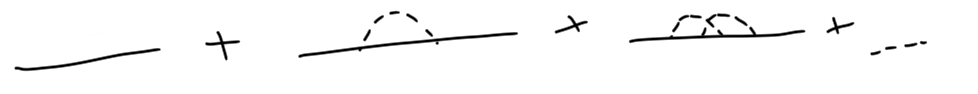
\includegraphics[scale=0.4]{lots.png}  \end{figure}

\noindent The end result if the sum of very many integrals of Wick contractions, and Feynman rules, dependent on the form of $\hat{H}_{int}$, are used to exploit patterns and cancellations in the terms. 

\subsection*{Example: Yukawa Theory}

\noindent Consider the Hamiltonian with interaction based on the fermion density $\hat{\bar{\psi}} \hat{\psi}$ and a single boson field $\hat{\phi}$, make the boson field sensitive to the density of the fermion field

\begin{equation}
\hat{H} =\hat{H}_{KG} + \hat{H}_{Dirac} + \int d^3 x \,\, g \, \hat{\bar{\psi}}(x) \hat{\psi}(x) \hat{\phi}(x).
\end{equation}

\noindent The Feynman rules in momentum space for this quantum field theory are, with dashed lines for bosons and solid lines for fermios

\begin{enumerate}
\item Propagators
	\subitem $\wick[offset=1.5em]{\c {\hat{\phi}(x)} \c {\hat{\phi}(y)}} = \frac{i}{p^2 - m_\phi^2 + i \epsilon} = $ \begin{figure}[H]\centering 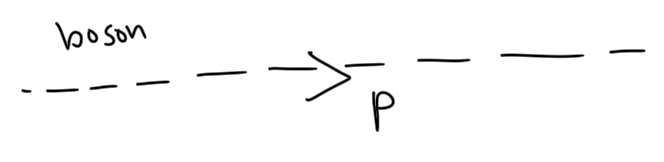
\includegraphics[scale=0.3]{bosonprop.png}  \end{figure}
	\subitem $\wick[offset=1.5em]{\c {\hat{\psi}(x)} \c {\hat{\bar{\psi}}(y)}} = \frac{i (\slashed{p} + m)}{p^2 - m^2 + i \epsilon} = $ \begin{figure}[H]\centering 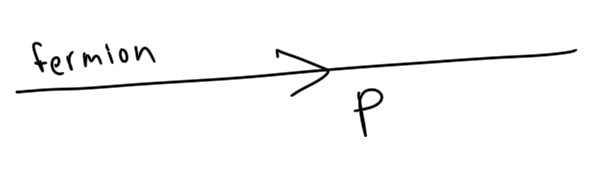
\includegraphics[scale=0.3]{fermionprop.png}  \end{figure}
\item Vertices
	\subitem $-ig = $ \begin{figure}[H]\centering 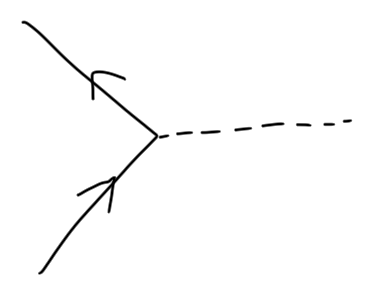
\includegraphics[scale=0.3]{vertex.png}  \end{figure}
\item External Legs
	\subitem $\wick[offset=1.5em]{\c {\hat{\phi}} \c {\ket{q}}} = 1 = $ \begin{figure}[H]\centering 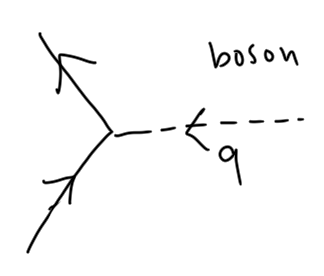
\includegraphics[scale=0.5]{bosonket.png}  \end{figure}
	\subitem $\wick[offset=1.5em]{\c {\bra{q}} \c {\hat{\phi}}} = 1 = $ \begin{figure}[H]\centering 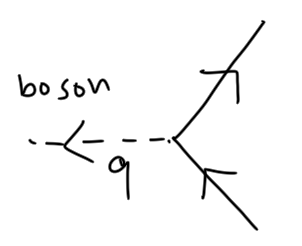
\includegraphics[scale=0.5]{bosonbra.png}  \end{figure}
	\subitem $\wick[offset=1.5em]{\c {\hat{\psi}} \c {\ket{p,s}}} = u^s (p) = $ \begin{figure}[H]\centering 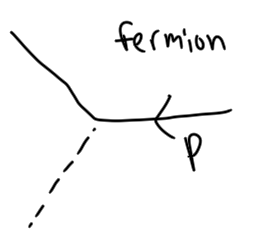
\includegraphics[scale=0.5]{fermionket.png}  \end{figure}
	\subitem $\wick[offset=1.5em]{\c {\bra{p,s}} \c {\hat{\bar{\psi}}}} = \bar{u}^s (p) = $ \begin{figure}[H]\centering 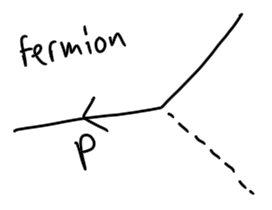
\includegraphics[scale=0.5]{fermionbra.png}  \end{figure}
	\subitem $\wick[offset=1.5em]{\c {\hat{\bar{\psi}}} \c {\ket{k,s}}} = \bar{v}^s (k) = $ \begin{figure}[H]\centering 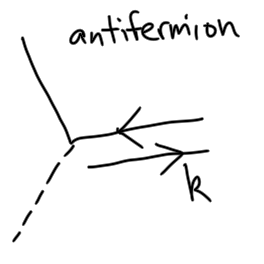
\includegraphics[scale=0.5]{antifermionket.png}  \end{figure}
	\subitem$ \wick[offset=1.5em]{\c {\bra{k,s}} \c {\hat{\psi}}} = v^s (k) = $ \begin{figure}[H]\centering 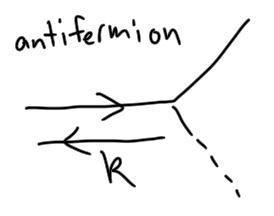
\includegraphics[scale=0.5]{antifermionbra.png}  \end{figure}
\item Conserve momentum at each vertex
\item Integrate over each loop momentum
\item Calculate the sign of the diagram
\item Divide by the symmetry factor
\end{enumerate}

\noindent Then the $n$-point Green's function is the sum of all connected and amputated Feynman diagrams with $n$ external legs subject to rules 1 through 7 above.

\noindent For example, a fermion scattering process looks like

\begin{figure}[H]\centering 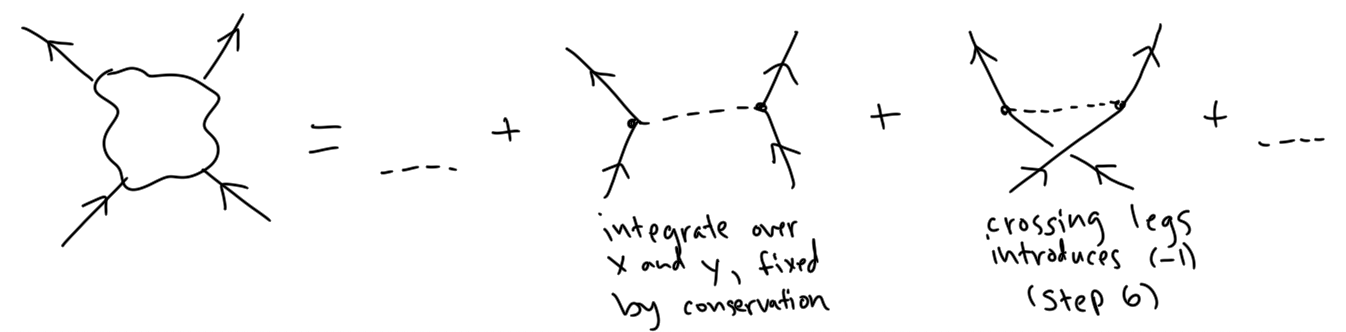
\includegraphics[scale=0.5]{fermionscattering.png}  \end{figure} 

\clearpage

\end{document}